\documentclass{121Temp}

\usepackage{amsmath}
\usepackage{amssymb}
\usepackage{amsthm}
\usepackage{commath}
\usepackage{listings}
\usepackage{mathtools}
\usepackage{float}

\usepackage{hyperref}

\usepackage{graphicx}
\graphicspath{ {images/} }

\hwauthor{Jonathan Levine}{jonlevi@sas.upenn.edu}
\hwcourse{BIBB 585}
\hwrecitation{401}
\hwno{2}

% \date{}  % uncomment this line to suppress the current date in the title
% \date{Due: Never}  % or uncomment this line to manually add a date
% \hwonelateday                   % uncomment either this line or the next to
% \hwtwolatedays                  % indicate that you are using an extension

\begin{document}
\maketitle

% Problem 1
\hwproblem
\label{Q1}
Give a short description of equation (5.25) including a description of the variables. Why do we use the
form n4 and m3h?

The equation for the membrane current, $i_m$ is equal to the sum of the currents for each ion. Given by Ohm's Law, this is $$i_m = \sum_{i}^{} g_i(V-E_i)$$
For the leakage current term, the conductance is constant, and thus the product is simply the product of the maximal conductance and the driving force $$i_L = \overline{g}_L(V-E_L)$$. For persistent, non-inactivating currents, the conductance is a function of voltage, and follows an activation function that depends on the probability of all subunits being in an open state simultaneously. Since there are roughly 4 subunits for the potassium channel, the probability is given as $n^4$, where n is the gating variable describing the voltage and time dependencies of the conductance. Therefore the potassium current in the equation is $$i_K = \overline{g}_Kn^4(V-E_K)$$. For Inactivating, transient conductances, we also need to model the inactivation gate as an independent process from the activation. We can similarly define h as the de-inactivation variable, and together with m (similar to n but this time for Sodium), we can describe the dynamics of sodium conductance as a function of voltage and time by describing its activation and de-inactivation through the m and h functions. One could make a similar argument about the exponents on the m and h terms relating to the number of independent events required for a full opening. The exponents were also chosen because they fit the experimental data best. At any rate, the sodium conductance can be modelled by $m^3h$, and thus the sodium current becomes $$i_{Na} = \overline{g}_{Na}m^3h(V-E_{Na})$$. Therefore we have $$i_m = \sum_{i}^{} g_i(V-E_i) $$ $$=i_L + i_K + i_{Na}$$ $$= \overline{g}(V-E_L) + \overline{g}_Kn^4(V-E_K) + \overline{g}_{Na}m^3h(V-E_{Na})$$

% Problem 2
\hwproblem
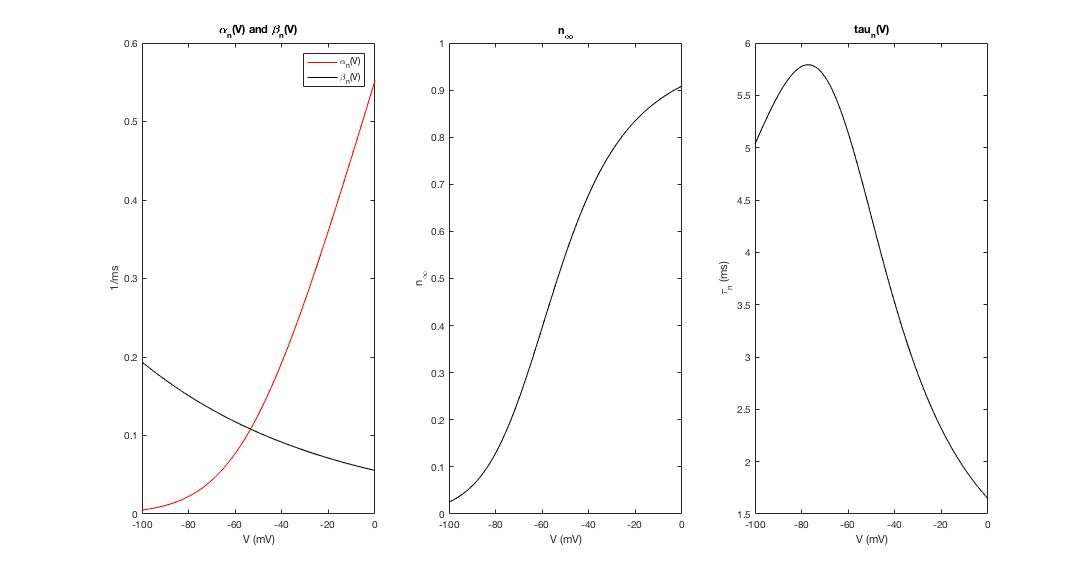
\includegraphics[scale=.35]{59}


% Problem 3
\hwproblem
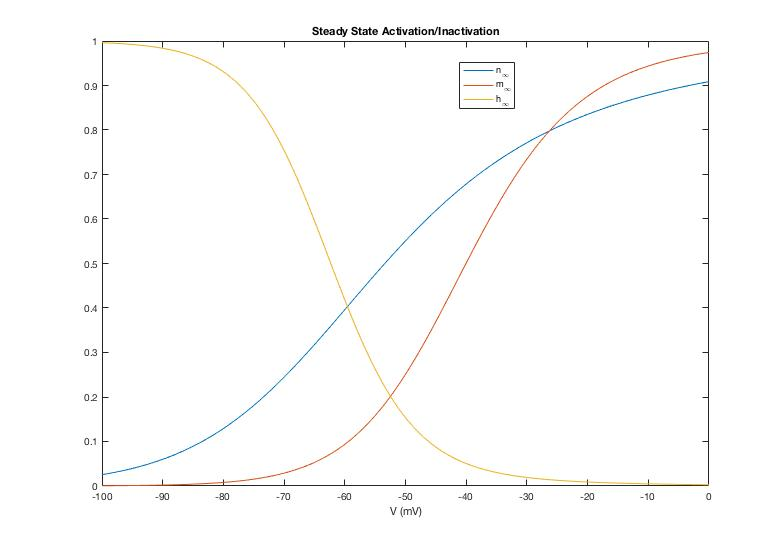
\includegraphics[scale=.55]{510a.jpg}
% Problem 4
\hwproblem
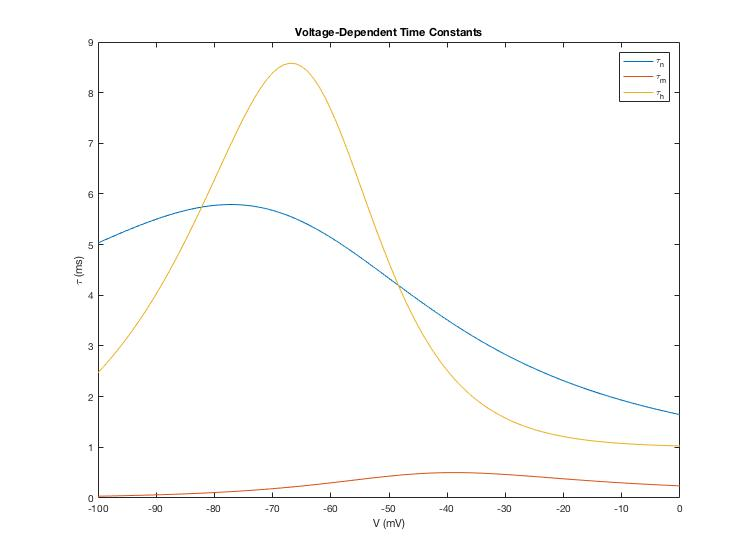
\includegraphics[scale=.55]{510b.jpg}

\hwproblem

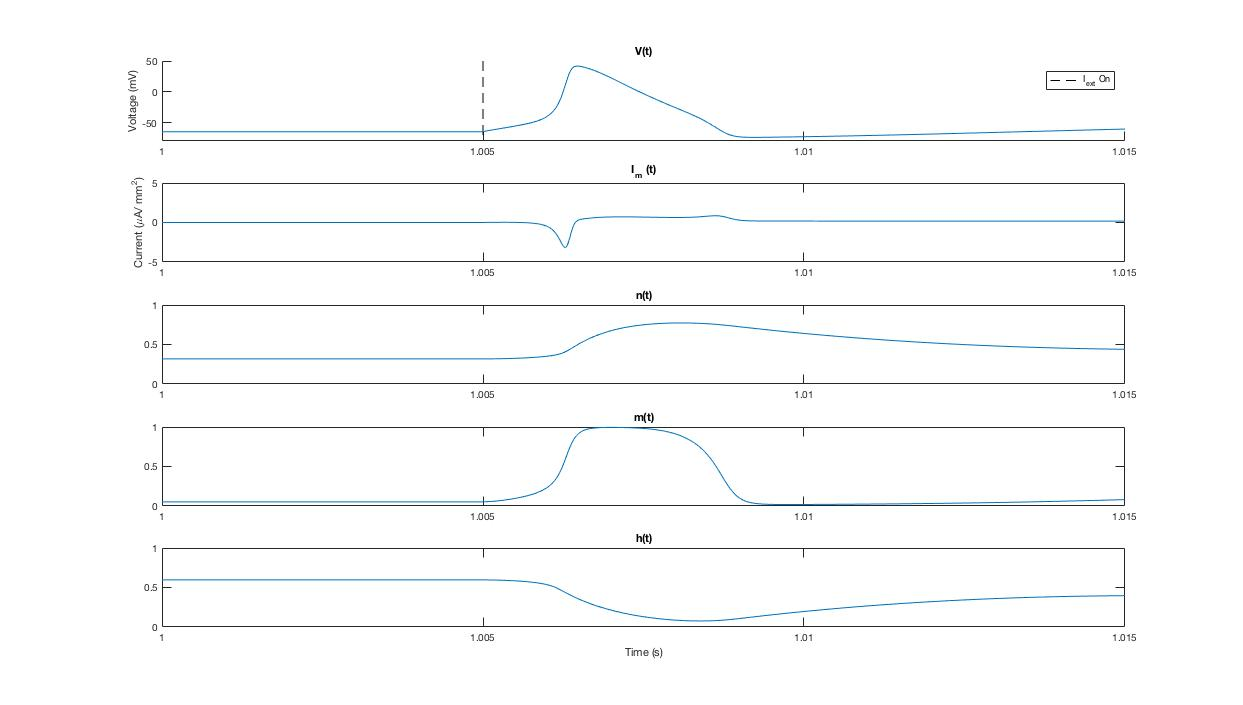
\includegraphics[scale=.45]{511.jpg}

\hwproblem
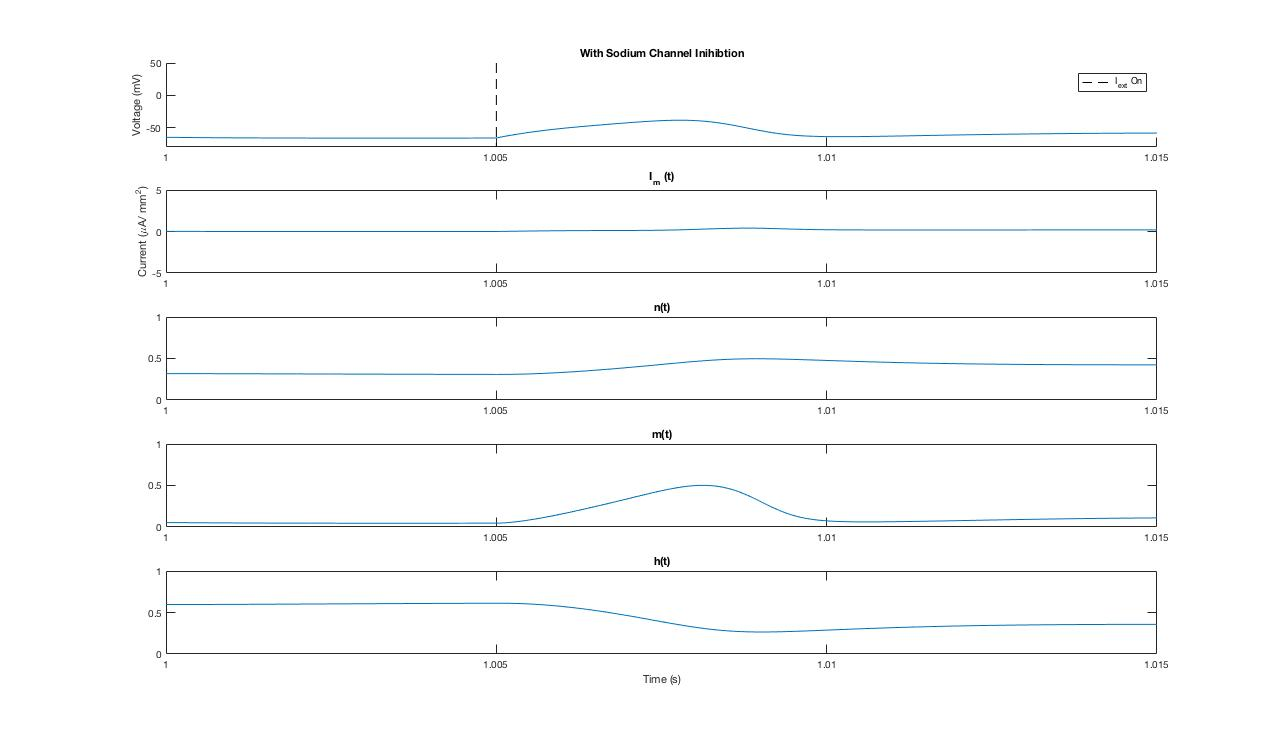
\includegraphics[scale=.45]{NaBlock.jpg}
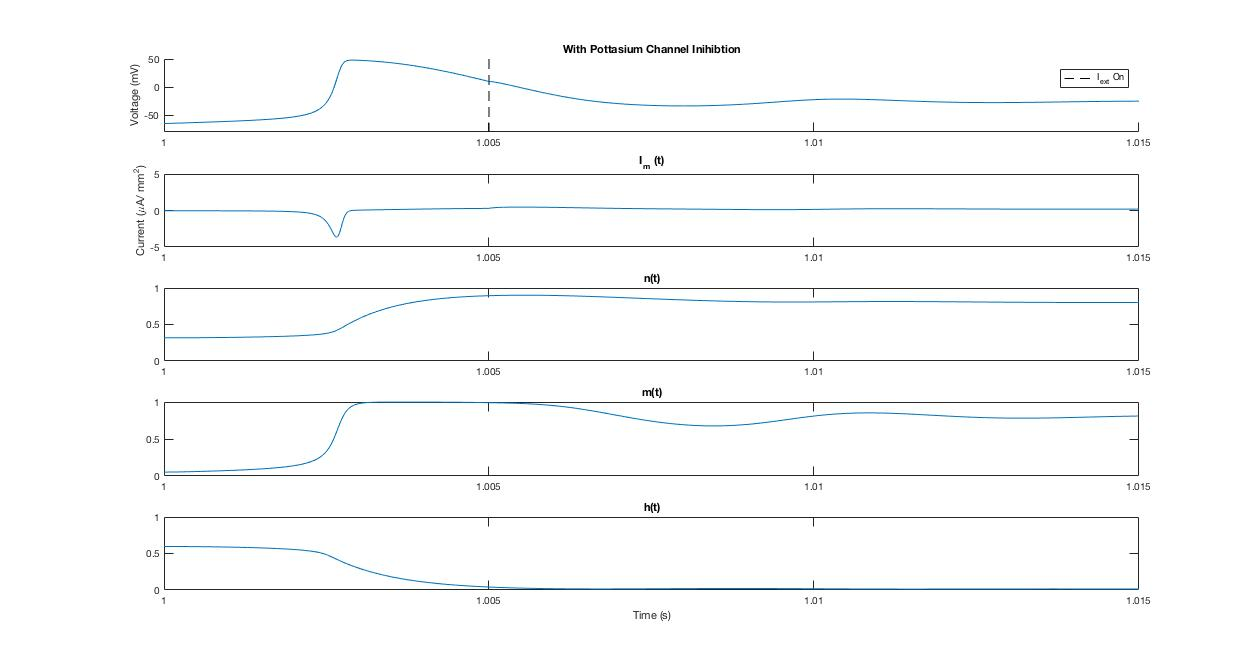
\includegraphics[scale=.45]{KBlock.jpg}
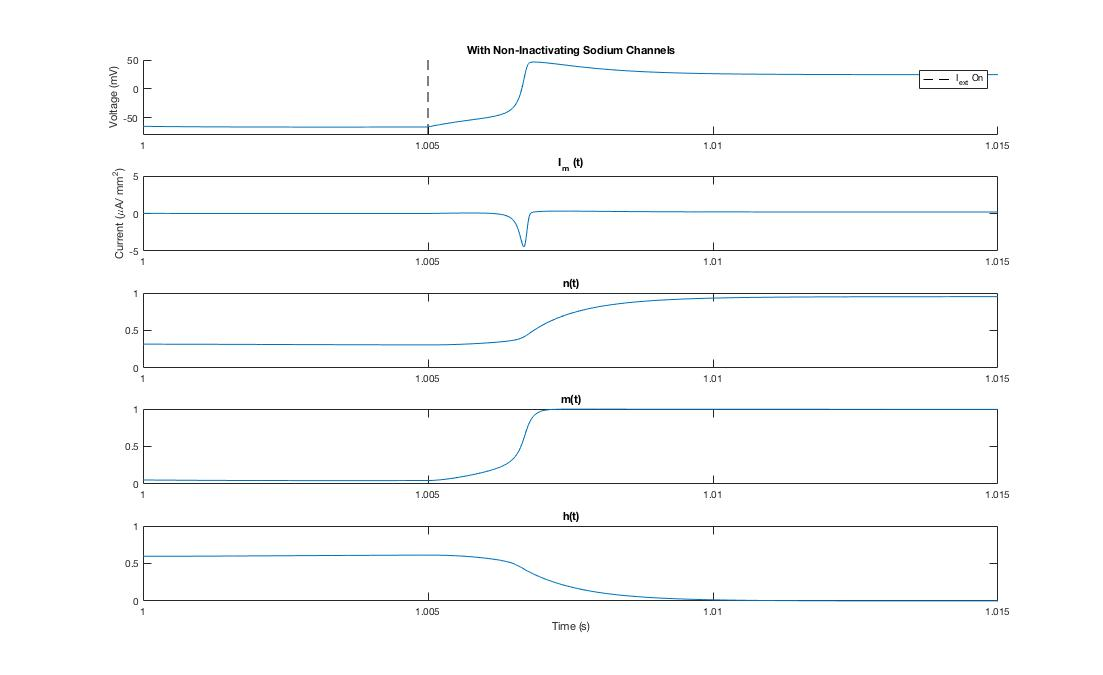
\includegraphics[scale=.45]{persistentNa.jpg}


\end{document}